%
% 
%
% Copyright (C) 1997-2011 by Dimitri van Heesch.
%
% Permission to use, copy, modify, and distribute this software and its
% documentation under the terms of the GNU General Public License is hereby 
% granted. No representations are made about the suitability of this software 
% for any purpose. It is provided "as is" without express or implied warranty.
% See the GNU General Public License for more details.
%
% Documents produced by Doxygen are derivative works derived from the
% input used in their production; they are not affected by this license.

\documentclass{book}
\usepackage[a4paper,left=2.5cm,right=2.5cm,top=2.5cm,bottom=2.5cm]{geometry}
\usepackage{makeidx}
\usepackage{natbib}
\usepackage{graphicx}
\usepackage{multicol}
\usepackage{float}
\usepackage{geometry}
\usepackage{listings}
\usepackage{color}
\usepackage{ifthen}
\usepackage[table]{xcolor}
\usepackage{textcomp}
\usepackage{alltt}
\usepackage{ifpdf}
\ifpdf
\usepackage[pdftex,
            pagebackref=true,
            colorlinks=true,
            linkcolor=blue,
            unicode
           ]{hyperref}
\else
\usepackage[ps2pdf,
            pagebackref=true,
            colorlinks=true,
            linkcolor=blue,
            unicode
           ]{hyperref}
\usepackage{pspicture}
\fi
\usepackage[utf8]{inputenc}
\usepackage{mathptmx}
\usepackage[scaled=.90]{helvet}
\usepackage{courier}
\usepackage{sectsty}
\usepackage[titles]{tocloft}
\usepackage{doxygen}
\lstset{language=C++,inputencoding=utf8,basicstyle=\footnotesize,breaklines=true,breakatwhitespace=true,tabsize=8,numbers=left }
\makeindex
\setcounter{tocdepth}{3}
\renewcommand{\footrulewidth}{0.4pt}
\renewcommand{\familydefault}{\sfdefault}
\renewcommand{\cftsecindent}{0 em}
\renewcommand{\cftsecnumwidth}{3.2 em}
\renewcommand{\cftsubsecindent}{3.2 em}
\newcommand{\thisyear}{\the\year}
\hfuzz=15pt
\setlength{\emergencystretch}{15pt}
\hbadness=750
\tolerance=750
\begin{document}
\begin{titlepage}
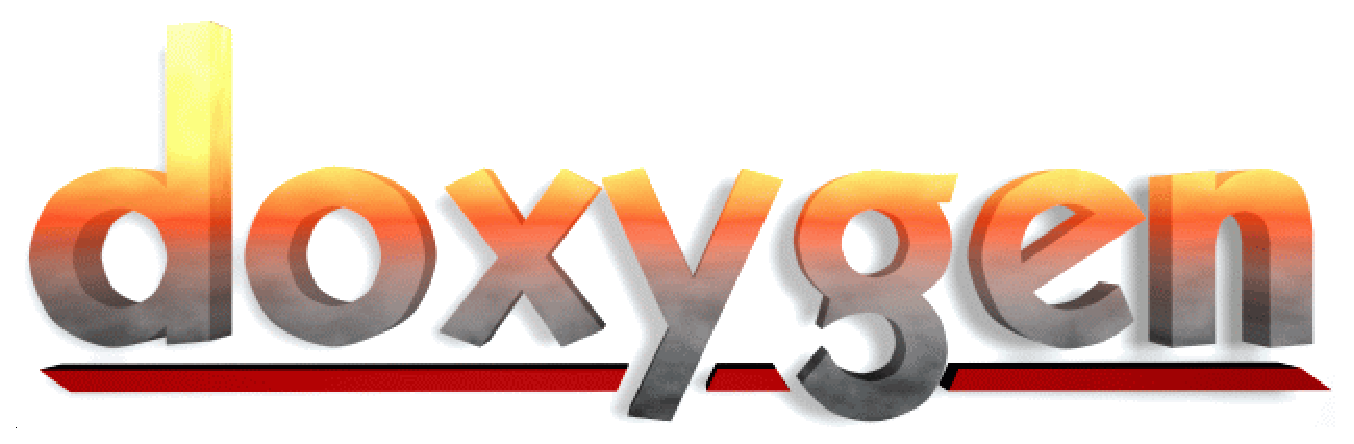
\includegraphics[width=\textwidth]{doxygen_logo}
\begin{center}
Manual for version $VERSION\\[2ex]
Written by Dimitri van Heesch\\[2ex]
\copyright 1997-\thisyear
\end{center}
\end{titlepage}
\clearemptydoublepage
\tableofcontents
\clearemptydoublepage
\pagenumbering{arabic}
\include{index}
\part{User Manual}
\chapter{Installation}\label{install}\hypertarget{install}{}\input{install}
\chapter{Getting Started}\label{starting}\hypertarget{starting}{}\input{starting}
\chapter{Documenting the code}\label{docblocks}\hypertarget{docblocks}{}\input{docblocks}
\chapter{Markdown}\label{markdown}\hypertarget{markdown}{}\input{markdown}
\chapter{Grouping}\label{grouping}\hypertarget{grouping}{}\input{grouping}
\chapter{Including Formulas}\label{formulas}\hypertarget{formulas}{}\input{formulas}
\chapter{Graphs and diagrams}\label{diagrams}\hypertarget{diagrams}{}PROJECT_NAME       = "Diagrams"
OUTPUT_DIRECTORY   = ../html/examples/diagrams
HAVE_DOT           = YES
EXTRACT_ALL        = YES
GENERATE_LATEX     = YES
GENERATE_MAN       = NO
GENERATE_RTF       = NO
CASE_SENSE_NAMES = NO
ENABLE_PREPROCESSING       = YES
INPUT              = .
STRIP_CODE_COMMENTS = NO
FILE_PATTERNS      = diagrams_*.h
QUIET              = YES
JAVADOC_AUTOBRIEF = YES
SEARCHENGINE     = NO
COMPACT_LATEX = YES
LATEX_HIDE_INDICES     = YES

\chapter{Preprocessing}\label{preprocessing}\hypertarget{preprocessing}{}\input{preprocessing}
\chapter{Automatic link generation}\label{autolink}\hypertarget{autolink}{}PROJECT_NAME     = "Automatic link generation"
OUTPUT_DIRECTORY = autolink
GENERATE_LATEX   = NO
GENERATE_MAN     = NO
GENERATE_RTF     = NO
CASE_SENSE_NAMES = NO
INPUT            = autolink.cpp
QUIET            = YES
JAVADOC_AUTOBRIEF = YES
SEARCHENGINE     = NO

\chapter{Output Formats}\label{output}\hypertarget{output}{}\input{output}
\chapter{Searching}\label{searching}\hypertarget{searching}{}\input{searching}
\chapter{Customizing the Output}\label{customize}\hypertarget{customize}{}\input{customize}
\chapter{Custom Commands}\label{custcmd}\hypertarget{custcmd}{}\input{custcmd}
\chapter{Link to external documentation}\label{external}\hypertarget{external}{}\input{external}
\chapter{Frequently Asked Questions}\label{faq}\hypertarget{faq}{}\input{faq}
\chapter{Troubleshooting}\label{trouble}\hypertarget{trouble}{}\input{trouble}
\part{Reference Manual}
\chapter{Features}\label{features}\hypertarget{features}{}\input{features}
\chapter{Doxygen usage}\label{doxygen_usage}\hypertarget{doxygen_usage}{}\input{doxygen_usage}
\chapter{Doxywizard usage}\label{doxywizard_usage}\hypertarget{doxywizard_usage}{}\input{doxywizard_usage}
\chapter{Configuration}\label{config}\hypertarget{config}{}\input{config}
\chapter{Special Commands}\label{commands}\hypertarget{commands}{}\input{commands}
\chapter{HTML commands}\label{htmlcmds}\hypertarget{htmlcmds}{}\input{htmlcmds}
\chapter{XML commands}\label{xmlcmds}\hypertarget{xmlcmds}{}\input{xmlcmds}
\part{Developers Manual}
\chapter{Doxygen's internals}\label{arch}\hypertarget{arch}{}\input{arch}
\chapter{Perl Module Output format}\label{perlmod}\hypertarget{perlmod}{}\input{perlmod}
\chapter{Internationalization}\label{langhowto}\hypertarget{langhowto}{}\input{langhowto}
\printindex
\end{document}
